%File Generated with PyPaper
\documentclass[aps,prl,reprint,amsmath,amssymb,superscriptaddress,notitlepage,groupedaddress,twocolumn]{revtex4-1}
\usepackage{graphicx}
\usepackage{dcolumn}
\usepackage{stackengine}
\usepackage[dvipsnames*,svgnames]{xcolor}
\usepackage{verbatim}
\usepackage[position=bottom,caption=false,captionskip=3pt,font=normalsize,subrefformat=simple,labelformat=simple]{subfig}
\renewcommand{\thesubfigure}{(\alph{subfigure})}
\usepackage{listings}
\usepackage{mathtools}
\usepackage{amsmath}
\usepackage{chngcntr}
\usepackage{bm}
\usepackage{url}
\def\UrlBreaks{\do\/\do-}
\newcommand {\framedgraphic}[2] {\begin{frame}{#1}\begin{center}\includegraphics[width=\textwidth,height=0.8\textheight,keepaspectratio]{#2}\end{center}\end{frame}}\usepackage[breaklinks]{hyperref}
\usepackage{breakurl}
\usepackage{tabularx}
\usepackage{soul}
\hypersetup{
colorlinks,
linkcolor={blue!100!black},
citecolor={blue},
urlcolor={blue!80!black}}
\lstset{basicstyle=\small\ttfamily,columns=flexible,breaklines=true}\newcommand{\fakesection}[1]{\par\refstepcounter{section}\sectionmark{#1}\addcontentsline{toc}{section}{\protect\numberline{\thesection}#1}}\def\equationautorefname~#1\null{#1\null}
\raggedbottom\usepackage[bottom]{footmisc} \makeatletter \def\p@section{} \def\p@subsubsection{} \makeatother\begin{document}
\title{Byesim: a tool for fast device characterization with Bayesian inference}
\author{Rachel Kurchin}
\affiliation{Department of Mechanical Engineering, Massachusetts Institute of Technology, 77 Massachusetts Avenue, Cambridge, MA 02139, USA}
\author{Giuseppe Romano}
\affiliation{Department of Mechanical Engineering, Massachusetts Institute of Technology, 77 Massachusetts Avenue, Cambridge, MA 02139, USA}
\author{Tonio Buonassisi}
\email{buonassi@mit.edu}
\affiliation{Department of Mechanical Engineering, Massachusetts Institute of Technology, 77 Massachusetts Avenue, Cambridge, MA 02139, USA}
\begin{abstract}
Achieving low thermal conductivity and good electrical properties is a crucial condition for thermal energy harvesting materials. Nanostructuring offers a very powerful tool to address both requirements: in nanostructured materials, boundaries preferentially scatter phonons compared to electrons. The search for low-thermal conductivity nanostructures is typically limited to materials with simple crystal structures, such as silicon, because of the complexity arising from modeling branch- and wave vector-dependent nanoscale heat transport. Using the phonon mean-free-path (MFP) dependent Boltzmann transport equation, a model that overcomes this limitation, we compute thermal transport in 75 nanoporous Half Heusler compounds for different pore sizes. We demonstrate that the optimization of thermal transport in nanostructures should take into account both bulk thermal properties and geometry-dependent phonon suppression, two aspects that are typically engineered separately. In fact, our work predicts that, given a set of bulk materials and a system geometry, the ordering of the bulk thermal conductivity does not necessarily align with that of the nanostructure. We show that what dictates thermal transport is the interplay between the bulk MFP distribution and the material's characteristic length. Finally, we derive a thermal transport model than enables fast systems screening within large bulk material repositories and a given geometry. Our study motivates the need for a holistic approach in engineering thermal transport and provides a method for high-throughput materials discovery.\end{abstract}
\maketitle

\section*{Acknowledgements}
Research supported as part of the Solid-State Solar-Thermal Energy Conversion Center (S3TEC), an Energy Frontier Research Center funded by the US Department of Energy (DOE), Office of Science, Basic Energy Sciences (BES), under Award DESC0001.\par 
\begin{equation}
\begin{split}\label{Eq:1001}
E=mc^2 
\end{split}
\end{equation}

\section*{Introduction}
Example of referencens as seen in ~\cite{fugallo2014thermal} and this refers to fig ~\subref*{Fig:10a}referes the Eq. ~(\autoref{Eq:1001}) 
\begin{figure*}[!ht]

\subfloat[\label{Fig:10a}]
{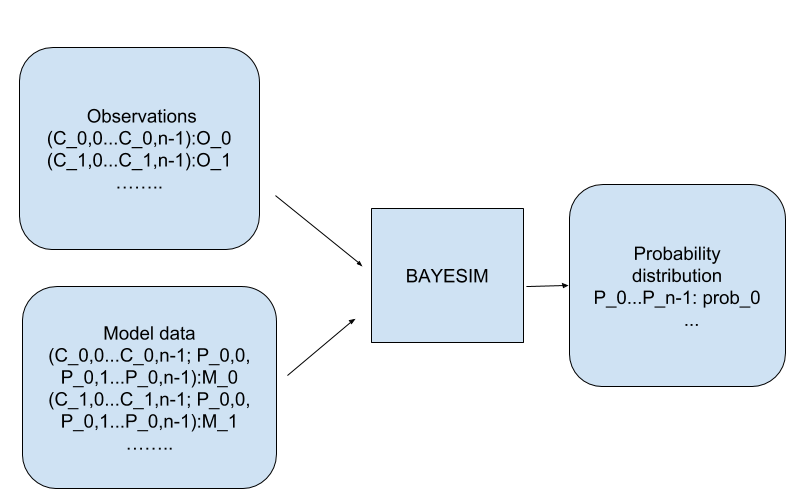
\includegraphics[width=0.48\textwidth]{./figure_1a.png}}
\hfill
\subfloat[\label{Fig:10b}]
{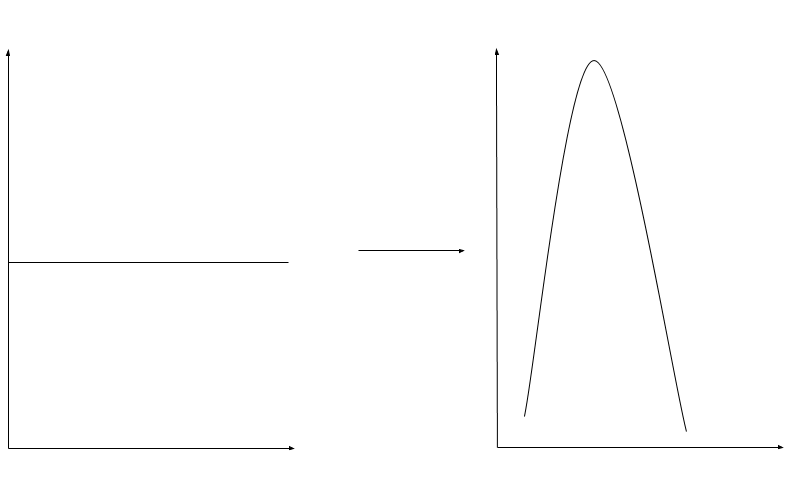
\includegraphics[width=0.48\textwidth]{./figure_1b.png}}
\caption{}
\end{figure*}
 %merlin.mbs apsrev4-1.bst 2010-07-25 4.21a (PWD, AO, DPC) hacked
%Control: key (0)
%Control: author (8) initials jnrlst
%Control: editor formatted (1) identically to author
%Control: production of article title (-1) disabled
%Control: page (0) single
%Control: year (1) truncated
%Control: production of eprint (0) enabled
\begin{thebibliography}{1}%
\makeatletter
\providecommand \@ifxundefined [1]{%
 \@ifx{#1\undefined}
}%
\providecommand \@ifnum [1]{%
 \ifnum #1\expandafter \@firstoftwo
 \else \expandafter \@secondoftwo
 \fi
}%
\providecommand \@ifx [1]{%
 \ifx #1\expandafter \@firstoftwo
 \else \expandafter \@secondoftwo
 \fi
}%
\providecommand \natexlab [1]{#1}%
\providecommand \enquote  [1]{``#1''}%
\providecommand \bibnamefont  [1]{#1}%
\providecommand \bibfnamefont [1]{#1}%
\providecommand \citenamefont [1]{#1}%
\providecommand \href@noop [0]{\@secondoftwo}%
\providecommand \href [0]{\begingroup \@sanitize@url \@href}%
\providecommand \@href[1]{\@@startlink{#1}\@@href}%
\providecommand \@@href[1]{\endgroup#1\@@endlink}%
\providecommand \@sanitize@url [0]{\catcode `\\12\catcode `\$12\catcode
  `\&12\catcode `\#12\catcode `\^12\catcode `\_12\catcode `\%12\relax}%
\providecommand \@@startlink[1]{}%
\providecommand \@@endlink[0]{}%
\providecommand \url  [0]{\begingroup\@sanitize@url \@url }%
\providecommand \@url [1]{\endgroup\@href {#1}{\urlprefix }}%
\providecommand \urlprefix  [0]{URL }%
\providecommand \Eprint [0]{\href }%
\providecommand \doibase [0]{http://dx.doi.org/}%
\providecommand \selectlanguage [0]{\@gobble}%
\providecommand \bibinfo  [0]{\@secondoftwo}%
\providecommand \bibfield  [0]{\@secondoftwo}%
\providecommand \translation [1]{[#1]}%
\providecommand \BibitemOpen [0]{}%
\providecommand \bibitemStop [0]{}%
\providecommand \bibitemNoStop [0]{.\EOS\space}%
\providecommand \EOS [0]{\spacefactor3000\relax}%
\providecommand \BibitemShut  [1]{\csname bibitem#1\endcsname}%
\let\auto@bib@innerbib\@empty
%</preamble>
\bibitem [{\citenamefont {Fugallo}\ \emph {et~al.}(2014)\citenamefont
  {Fugallo}, \citenamefont {Cepellotti}, \citenamefont {Paulatto},
  \citenamefont {Lazzeri}, \citenamefont {Marzari},\ and\ \citenamefont
  {Mauri}}]{fugallo2014thermal}%
  \BibitemOpen
  \bibfield  {author} {\bibinfo {author} {\bibfnamefont {G.}~\bibnamefont
  {Fugallo}}, \bibinfo {author} {\bibfnamefont {A.}~\bibnamefont {Cepellotti}},
  \bibinfo {author} {\bibfnamefont {L.}~\bibnamefont {Paulatto}}, \bibinfo
  {author} {\bibfnamefont {M.}~\bibnamefont {Lazzeri}}, \bibinfo {author}
  {\bibfnamefont {N.}~\bibnamefont {Marzari}}, \ and\ \bibinfo {author}
  {\bibfnamefont {F.}~\bibnamefont {Mauri}},\ }\href@noop {} {\bibfield
  {journal} {\bibinfo  {journal} {Nano letters}\ }\textbf {\bibinfo {volume}
  {14}},\ \bibinfo {pages} {6109} (\bibinfo {year} {2014})}\BibitemShut
  {NoStop}%
\end{thebibliography}%
\end{document}
